%% ----------------------------------------------------------------
%% Chapter 4: Spanwise-averaged Navier--Stokes equations
%% ----------------------------------------------------------------
%!TeX root = subfile
\label{chapter:sans}
\documentclass[../main.tex]{subfiles}
% ---------------------------------------------------------------- 
\begin{document}

\vspace{0.25cm}
Simulations of turbulent fluid flow around long cylindrical structures are computationally expensive because of the vast range of length scales, requiring simplifications such as dimensional reduction.
Current dimensionality reduction techniques such as strip-theory and depth-averaged methods do not take into account the natural flow dissipation mechanism inherent in the small-scale 3-D vortical structures.
In this chapter, a novel flow decomposition based on a local spanwise average of the flow is proposed, yielding the spanwise-averaged Navier--Stokes (SANS) equations.
The SANS equations include closure terms accounting for the 3-D effects otherwise not considered in 2-D formulations.
The SSR tensor modifies the flow dynamics from standard 2-D Navier--Stokes to spanwise-averaged dynamics.
It is shown that the SANS perfect closure recovers the unsteady spanwise-averaged solution of the Taylor--Green vortex and flow past a circular cylinder at $Re=10^4$.
Finally, it is demonstrated that eddy-viscosity models (EVMs) are not suited for the prediction of the spanwise stresses, motivating the need of a different closure as proposed in the following chapter.

\section{Introduction and literature review}

The vast range of spatial and temporal scales inherent in turbulence renders direct numerical simulations of most engineering and environmental flows impossible.
This is because the required resolution is governed by the balance of the flow convective and viscous forces, quantified by the Reynolds number.
For illustration, turbulent engineering or atmospheric flows have $Re\smallgtrsim 10^6-10^{10}$ and, as reviewed in \sref{sec:turbulence_cost}, directly simulating homogeneous isotropic turbulence in an $L^3$ box for one convection cycle would require $O(Re^3)$ operations \citep[p. 346]{Coleman2010,Pope2000}.
To avoid resolving the smallest time and length scales, turbulence models such as RANS, LES, and others have been developed to account for the unresolved scales of motion on coarse discretisations.

However, in many cases the scale of the flow is so large that turbulence models do not sufficiently reduce the computational cost and further simplifications are required, such as reducing the flow from three spatial dimensions down to two.
In the case of very long slender bodies, strip theory can be used to place 2-D strips along the structure span, reducing cost by orders of magnitude.
In offshore engineering, strip-theory methods have been used to simulate the vortex-induced vibrations of marine risers \citep{Herfjord1999}. \cite{Willden2001} considered a marine riser at a low Reynolds regime where the strips were linked by an inviscid unsteady 3-D vortex lattice.
Further investigations on marine risers multi-modal VIV phenomena were performed by the previous authors considering a more realistic Reynolds number ($\mathcal{O}(10^5)$) and including a LES turbulence model for the 2-D strips \citep{Willden2004}.
Other authors such as \cite{Yamamoto2004, Meneghini2004, Sun2012} employed a strip-theory discrete-vortex method to study the VIV phenomena on marine risers with $L_z/D=400$ and $Re=10^5$, modelling the flow viscous effects through an exponentially decaying function.
Other slender-body problems tackled with strip theory are found in naval engineering to simulate ship hydrodynamics \citep{Newman1979}, or in aerospace engineering for wing fluttering prediction \citep{Yates1966}.
A different dimensionality reduction technique is the depth-averaged method, typically used in the simulation of shallow open-channel flow such as rivers \citep{Molls1995}, where the dimensions of the problem are simplified by averaging along the shear direction of the flow.

The main shortcoming of the dimensionality reduction methods above is that the fluid dynamics of 2-D systems are intrinsically different from their 3-D counterparts.
In particular, 3-D turbulence cannot develop when the spanwise dimension is neglected.
Instead, 2-D turbulence promotes coherent and high-intensity vortices via vortex-thinning and vortex-merging events \citep{Xiao2009} ultimately inducing larger forces to the cylinder \citep{Mittal1995, Norberg2003}.
Because of this, these methods require additional dissipation mechanisms, often in the form of LES Smagorinsky models.
These turbulence models applied to 2-D systems decrease the vortices intensity thus inducing weaker forces on solid structures which can resemble those found in 3-D cases.
However, the dissipation mechanism is arbitrary and we show that it cannot be used to simulate 3-D turbulence dynamics in a 2-D simulation.

To address this issue, Bao et al. \citep{Bao2016, Bao2019} proposed a \textit{thick} strip-theory method, as hinted in \cite{Herfjord1999}.
Providing spanwise thickness to the strips allows the flow to locally develop 3-D turbulence, thus recovering the natural dissipation mechanism.
However, the minimum strip thickness at which 3-D turbulence dominates the flow is in the order of the structure diameter \citep{Bao2016,Font2019}, as discussed in \cref{chapter:jfm2019}. Hence, the inclusion of 3-D effects comes at the expense of increased computational cost, which can limit the simulation of realistic spans or Reynolds regimes. 

In this work, we propose a novel flow decomposition which separates the spanwise-averaged and the spanwise-fluctuating parts of the flow.
Instead of directly resolving the 3-D spatial scales, these are taken into account with an additional spanwise-fluctuating term inserted into the 2-D governing equations.
We call the resulting system of equations the spanwise-averaged Navier--Stokes equations (SANS).
In contrast to RANS or LES, the closure terms account for the 3-D turbulence effects enabling the simulation of turbulent wake flows in two dimensions.
Similarities can be drawn with depth-averaged methods.
Uniquely, the SANS equations do not assume hydrostatic pressure or approximately uniform velocity, instead being developed specifically to deal with fully 3-D wake turbulence.
Unlike RANS simulations, which can only (at best) reproduce the time-averaged forces, the SANS system is capable of reproducing the instantaneous spanwise-integrated forces on a locally cylindrical body. 
As such, a SANS strip theory is ideal for predicting the 3-D fluid-structure interactions with widely spaced 2-D simulation planes (see \fref{fig:strips}).

\begin{figure}[t]
\centering
\includegraphics[width=0.9\linewidth]{chapter4/strips/strips2}
\caption{
Sketch of the spanwise-averaged strip-theory method.
The original $L_z$ span is decomposed into multiple $L_a$ spanwise segments for which the SANS equations are simultaneously solved, hence reducing the computational domain (coloured region).
Solving the SANS equations for every spanwise-averaged strip allows to recover the local integrated forces induced to the cylinder.
The 2-D strips can be linked with a structural dynamic model similarly to \cite{Bao2016, Bao2019}.}
\label{fig:strips}
\end{figure}

\section{The spanwise-averaged Navier--Stokes equations}\label{sec:SANS_eqs}

When a flow is essentially homogeneous in one direction, this can be exploited to simplify modelling in a number of ways;
the turbulent flow statistics are invariant to translation along the homogeneous direction, there are no mean flow gradients in the homogeneous direction, and the component of mean velocity in the homogeneous direction can always be set 0 in an appropriate reference frame \citep[p. 76]{Pope2000}.
Therefore, a single homogeneous direction can be used to reduce a 3-D flow to a 2-D system of equations, potentially reducing the cost of simulation by orders of magnitude.

\subsection{Mathematical description} \label{sec:sans_math}

Starting from the conservation form of the non-dimensional 3-D Navier--Stokes momentum equations
\begin{equation}
\partial_t\vect{u}+\nabla \cdot \pars{\vect{u}\otimes\vect{u}}=-\nabla p+Re^{-1}\nabla^2\vect{u},\label{eq:N-S}
\end{equation}
the velocity vector field $\vect{u}\pars{\vect{x},t}=\pars{u,v,w}$ and the pressure scalar field $p\pars{\vect{x},t}$ are decomposed into a spanwise-averaged and a spanwise-fluctuating part as follows
\begin{equation}
q(\vect{x},t) = \avg{q}(x,y,t)+q\p(x,y,z,t),
\end{equation}
where $\avg{\cdot}$ and $(\cdot)\p$ denote the averaged and the fluctuating parts of the decomposition, respectively.
The average, also noted as $\avg{q}=Q$, can be defined on a $z\in\left[a,b\right]$ interval as
\begin{equation}
Q=\avg{q}\pars{x,y,t} = \frac{1}{b-a}\int^b_a q\pars{x,y,z,t}\,\mathrm{d}z.
\label{eq:spanwise_average}
\end{equation}
Such decomposition applied to the $\vect{e}_x$ component of \eref{eq:N-S} yields
\begin{gather}
\partial_t\pars{U+u\p}+\partial_x\pars{UU+2Uu\p+u\p u\p}+\partial_y\pars{VU+Vu\p+v\p U+v\p u\p}+\nonumber\\
+\partial_z\pars{WU+Wu\p+w\p U+w\p u\p}=\nonumber\\
=-\partial_x\pars{P+p\p}+Re^{-1}\left[\partial_{xx}\pars{U+u\p}+\partial_{yy}\pars{U+u\p}+\partial_{zz}\pars{U+u\p}\right].
\label{eq:N-S_decomp}
\end{gather}

Next, the following relations arising from \eref{eq:spanwise_average} are considered,
\begin{alignat}{3}
&\,\,q=Q+q\p,                      &&\qquad \,\,s=S+s\p,                       &&\qquad \avg{q+s}=Q+S,              \label{eq:rule1}\\
&\avg{Q}=Q,                  &&\qquad \avg{q\p}=0,                             &&\qquad \avg{Qs\p}=Q\avg{s\p}=0,      \label{eq:rule2} \\
&\avg{q\p q\p} \neq0,                    &&\qquad \avg{\partial_z q}\neq\partial_zQ, &&\qquad \,\,\partial_zQ=0,                \\
&\avg{\partial_t q} =\partial_t Q, &&\qquad \avg{\partial_x q} =\partial_x Q,  &&\qquad \avg{\partial_y q} =\partial_y Q.\label{eq:rule3}
\end{alignat}
Note that the spanwise average does not commute with the spanwise derivative, i.e. $\avg{\partial_z q}=\avg{\partial_z q\p}\neq\partial_zQ$, since the average and the derivative operate over the same variable $z$.
However, terms such as $\avg{\partial_z^n q}$ vanish under infinitely-long (periodic) averaging intervals, as discussed in \sref{sec:spanwise-periodic_interval}.

Applying the averaging operator to the whole \eref{eq:N-S_decomp} and considering the relations from \eref{eq:rule1} to \eref{eq:rule1} yields the governing equation of $U$,
\begin{gather}
\partial_tU+\partial_x\pars{UU+\avg{u\p u\p}}+\partial_y\pars{VU+\avg{v\p u\p}}+\avg{\partial_z\pars{Wu\p+w\p U+w\p u\p}}=\nonumber \\
=-\partial_xP+Re^{-1}\pars{\partial_{xx}U+\partial_{yy}U+\avg{\partial_{zz} u\p}}, \\
\partial_tU+\partial_x\pars{UU}+\partial_y\pars{VU}+U\avg{\partial_z w\p}=-\partial_xP+Re^{-1}\pars{\partial_{xx}U+\partial_{yy}U}-\nonumber\\
-\partial_x\avg{u\p u\p}-\partial_y\avg{v\p u\p}-W\avg{\partial_z u\p}-\avg{\partial_z\pars{w\p u\p}}+Re^{-1}\avg{\partial_{zz} u\p}. \label{eq:N-S_decom_avg}
\end{gather}

In order to rewrite \eref{eq:N-S_decom_avg} in its non-conservation form, the continuity equation is considered
\begin{equation}
\nabla\cdot\vect{u}=0, \label{eq:cont}
\end{equation}
and applying the same decomposing and averaging procedure yields
\begin{equation}
\partial_xU+\partial_yV+\avg{\partial_z w\p}=0.\label{eq:cont_decomp_avg}
\end{equation}
By substituting \eref{eq:cont_decomp_avg} into \eref{eq:N-S_decom_avg}, the non-conservation form is obtained and the $U\avg{\partial_z w\p}$ term vanishes yielding
\begin{gather}
\partial_tU+U\partial_xU+V\partial_yU=-\partial_xP+Re^{-1}\pars{\partial_{xx}U+\partial_{yy}U}-\partial_x\avg{u\p u\p}-\partial_y\avg{v\p u\p}-\nonumber\\
-W\avg{\partial_z u\p}-\avg{\partial_z\pars{w\p u\p}}+Re^{-1}\avg{\partial_{zz} u\p}.\label{eq:z-avg_X}
\end{gather}

Analogously to the spanwise decomposition for the $\vect{e}_x$ component of the momentum equations, the same procedure can be applied to the $\vect{e}_y$ and $\vect{e}_z$ components which respectively leads to
\begin{gather}
\partial_tV+U\partial_xV+V\partial_yV=-\partial_yP+Re^{-1}\pars{\partial_{xx}V+\partial_{yy}V}-\partial_x\avg{u\p v\p}-\partial_y\avg{v\p v\p}-\nonumber\\
-W\avg{\partial_z v\p}-\avg{\partial_z\pars{w\p v\p}}+Re^{-1}\avg{\partial_{zz} v\p},\\
\partial_tW+U\partial_xW+V\partial_yW=-\avg{\partial_z p\p}+Re^{-1}\pars{\partial_{xx}W+\partial_{yy}W}-\partial_x\avg{u\p w\p}-\partial_y\avg{v\p w\p}-\nonumber\\
-W\avg{\partial_z w\p}-\avg{\partial_z\pars{w\p w\p}}+Re^{-1}\avg{\partial_{zz} w\p}.\label{eq:z-avg_Z}
\end{gather}
Note that Eqs. \ref{eq:z-avg_X} to \ref{eq:z-avg_Z} are the 2-D incompressible Navier--Stokes equations with additional spanwise-fluctuating closure terms (first line, also referred in future mentions as ``spanwise stresses'') and terms arising from the finite spanwise-averaging length (second line).

With this, the complete 2-D SANS momentum equations can be written in a more compact form as
\begin{gather}
\partial_t\vect{U}+\vect{U}\cdot\nabla\vect{U}=-\nabla P+Re^{-1}\nabla^2\vect{U}-\nabla\cdot\boldsymbol\tau_{ij}^R-\nonumber\\
-W\avg{\partial_z \vect{u}\p}-\avg{\partial_z\pars{w\p \vect{u}\p}}+Re^{-1}\avg{\partial_{zz}\vect{u}\p},\label{eq:sans_full}
\end{gather}
where $\vect{U}=\pars{U,V}$, and the spanwise-stress residual (SSR) tensor $\boldsymbol\tau_{ij}^R$ is defined as
\begin{equation}
\boldsymbol\tau_{ij}^R= \avg{\vect{u}\otimes\vect{u}}-\avg{\vect{u}}\otimes\avg{\vect{u}} =
  \begin{pmatrix}
    \avg{u\p u\p} & \avg{u\p v\p} \\
    \avg{u\p v\p} & \avg{v\p v\p} 
  \end{pmatrix}.
\end{equation}

For the sake of completeness, the analogous spanwise-averaged VTE derivation is included in \aref{sec:savte}, where the relation between the velocity-velocity and vorticity-velocity spanwise stresses is derived as well.

\section{Columnar vortex between two infinite parallel plates}

The SANS equations dynamics is explored for an analytical test case where a known solution exists.
For this, a columnar vortex between two infinite parallel plates is considered \citep{Marshall2001}.
Marshall's analytical test case shows the stretching of a vortex tube by the superposition of an external straining field (\fref{fig:columnar_vortex}).

In a cylindrical coordinate system, we consider unit vectors $\vect{e}_r,\vect{e}_\theta,\vect{e}_z$ and define the vector fields $\vect{u}=\left(u_r,u_\theta,u_z\right),\,\boldsymbol\omega=\left(\omega_r,\omega_\theta,\omega_z\right)$ in a $\vect{x}=\left(r,\theta,z\right)$ cylindrical space. In this coordinate system, a columnar vortex is defined as
\begin{equation}
{\boldsymbol\omega_v}\pars{\vect{x},t}=\begin{cases}
\begin{array}{c}
\omega\left(t\right)\vect{e}_3\\
0
\end{array} & \begin{array}{c}
r\leq R\left(t\right),\\
r>R\left(t\right),
\end{array}\end{cases}
\end{equation}
where uniform vorticity within the vortex core is considered for the $\vect{e}_3$ direction.
Also note that the subscript $(\cdot)_v$ refers to the columnar vortex field.
The velocity field associated to the columnar vortex is
\begin{equation}
{\vect{u}_v}\pars{\vect{x},t}=\left(0,v\left(r,t\right),0\right).
\end{equation}

Next, we demonstrate that the superposition of an axisymmetric straining field to the vortex tube increases the vorticity magnitude (for incompressible flow) as a result of the vortex-stretching mechanism.
Let us consider the following straining field
\begin{equation}
\vect{u}_s=\pars{-\frac{\gamma r}{2},0,\gamma z},\label{eq:strain_field}
\end{equation}
where $\gamma$ is the rate of strain $(dL/dt=\gamma L_0)$, and the subscript $(\cdot)_s$ refers to the straining field.
Note that the straining field is irrotational, $\nabla\times\vect{u}_s=0$, so no vorticity is added.
With this, the superposition of the columnar vortex and the straining field results into the following vorticity and velocity fields, respectively
\begin{gather}
\boldsymbol\omega=\boldsymbol\omega_v=\pars{0,0,\omega(t)}\label{eq:vorticity_field}\\
\vect{u}=\vect{u}_v+\vect{u}_s=\pars{-\frac{\gamma r}{2},v(r,t),\gamma z}.\label{eq:velocity_field}
\end{gather}

\begin{figure}[!t]
    \centering
    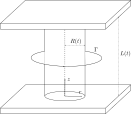
\includegraphics[width=0.45\textwidth]{chapter4/columnar_vortex/columnar_vortex}
    \caption{Columnar vortex of radius $R$ between two infinite parallel plates.
Adapted from \cite{Marshall2001}.}
    \label{fig:columnar_vortex}
\end{figure}

Substituting \eref{eq:vorticity_field} and \eref{eq:velocity_field} into the $\vect{e}_3$ component of the non-dimensional VTE, written in cylindrical coordinates as
\begin{gather}
\frac{\partial\omega_{z}}{\partial t}+u_r\frac{\partial \omega_{z}}{\partial r}+\frac{u_{\theta}}{r}\frac{\partial \omega_{z}}{\partial\theta}+u_z\frac{\partial \omega_{z}}{\partial z}=\omega_r\frac{\partial u_z}{\partial r}+\frac{\omega_{\theta}}{r}\frac{\partial u_z}{\partial\theta}+\omega_{z}\frac{\partial u_z}{\partial z}+\nonumber\\
+\frac{1}{Re}\left(\frac{\partial^{2}\omega_{z}}{\partial r^{2}}+\frac{1}{r}\frac{\partial\omega_{z}}{\partial r}+\frac{1}{r^{2}}\frac{\partial^{2}\omega_{z}}{\partial\theta^{2}}+\frac{\partial^{2}\omega_{z}}{\partial z^{2}}\right),\label{eq:vte_cyl_non_conserv}
\end{gather}
yields
\begin{gather}
\pd{\omega}{t}+0+0+0=0+0+\omega\frac{\partial}{\partial z}\pars{\gamma z}+0+...+0,\\
\dd{\omega}{t}=\gamma\omega.
\end{gather}
Therefore, it is shown that an increase in the straining field $\left(\gamma>0\right)$ induces an increase of the vorticity magnitude (vortex-stretching), and a decrease in the straining field $\left(\gamma<0\right)$ induces a decrease of the vorticity magnitude (vortex-compression).
Also note that the $\gamma\omega$ term arises from  $\omega_{z}\left(\partial u_{z}/\partial z\right)$, indeed part of the vortex-stretching term.

Next, the Marshall's vortex stretching analytical test case is considered using the spanwise-averaged VTE.
In cylindrical coordinates, the non-dimensional spanwise-averaged VTE can be written as (see derivation in \sref{sec:cyl_coords})
\begin{gather}
\pd{\Omega_z}{t}+U_r\pd{\Omega_z}{r}+\frac{U_\theta}{r}\pd{\Omega_z}{\theta}=\Omega_r\pd{U_z}{r}+\frac{\Omega_\theta}{r}\pd{U_z}{\theta}+\frac{1}{Re}\pars{\ddn{\Omega_z}{r}{2}+\frac{1}{r}\pd{\Omega_z}{r}+\frac{1}{r^2}\ddn{\Omega_z}{\theta}{2}}\nonumber\\
-\frac{1}{r}\bracs{\pd{}{r}\pars{\avg{r u_r\p\omega_z\p}-\avg{r \omega_r\p u_z\p}}+
\pd{}{\theta}\pars{\avg{u_\theta\p\omega_z\p}-\avg{\omega_\theta\p u_z\p}}}+\nonumber\\
+\Omega_z\avg{\pd{u_z\p}{z}}-U_z\avg{\pd{\omega_z\p}{z}}+\frac{1}{Re}\avg{\ddn{\omega_z\p}{z}{2}}.\label{eq:vte_cyl_avg}
\end{gather}

Applying the averaging procedure to the velocity field resulting from the superposition of the columnar vortex and the straining field (\eref{eq:velocity_field}) yields
\begin{gather}
\vect{u}=\left(-\frac{\gamma r}{2},0,\gamma z\right),\\
U_r =\frac{1}{b-a}\int^b_a -\frac{\gamma r}{2}\,dz=-\frac{\gamma r}{2},\quad u_r\p=0,\\
U_z =\frac{1}{b-a}\int^b_a \gamma z\,dz=\gamma\frac{a+b}{2},\quad u_z\p=u_z-U_z=\gamma\pars{z-\frac{a+b}{2}},\\
\vect{U}=\pars{-\frac{\gamma r}{2},0,\gamma\frac{a+b}{2}},
\end{gather}	
while the vorticity field stays as $\vect{\Omega}=\pars{0,0,\omega(t)}$.
Substituting the averaged and fluctuating parts of the velocity and the vorticity fields into \eref{eq:vte_cyl_avg} yields
\begin{gather}
\pd{\omega}{t}+0+0=0+0+...+\omega\frac{\partial}{\partial z}\pars{\gamma z}+0+...+0,\\
\dd{\omega}{t}=\gamma\omega.
\end{gather}
This shows that the vortex-stretching mechanism is still present in the spanwise-averaged VTE.
However, note that $\gamma\omega$ arises from $\Omega_z \avg{\partial_z u_z\p}$, a term that vanishes when an infinite (spanwise-periodic) averaging interval is considered, as explained next.

\section{Averaging over a spanwise-periodic interval} \label{sec:spanwise-periodic_interval}

The SANS equations can be greatly simplified when the averaging is performed over a periodic interval since
\begin{equation}
\avg{\partial_z q} = \avg{\partial_z q\p}  =\frac{1}{b-a}\int^b_a \frac{\partial q\p}{\partial z}\,dz=\frac{q\p\left(b\right)-q\p\left(a\right)}{b-a}=0
\label{eq:periodic_assumption}
\end{equation}
because $q\p(a)=q\p(b)$.
This yields a simplified version of SANS which can be written as
\begin{gather}
\partial_tU+U\partial_xU+V\partial_yU=-\partial_xP+Re^{-1}\pars{\partial_{xx}U+\partial_{yy}U}-\partial_x\avg{u\p u\p}-\partial_y\avg{v\p u\p},\\
\partial_tV+U\partial_xV+V\partial_yV=-\partial_yP+Re^{-1}\pars{\partial_{xx}V+\partial_{yy}V}-\partial_x\avg{u\p v\p}-\partial_y\avg{v\p v\p},\\
\partial_tW+U\partial_xW+V\partial_yW=Re^{-1}\pars{\partial_{xx}W+\partial_{yy}W}-\partial_x\avg{u\p w\p}-\partial_y\avg{v\p w\p}.
\end{gather}
Note that the spatial dependency on the spanwise direction is lost during the process (there are no $z$ derivatives present in the final form), and also the momentum equations for $U$ and $V$ are decoupled from $W$.
The momentum equation for $W$ becomes a convective-diffusive equation (with additional forcing terms) since the pressure term vanishes under the assumption of spanwise periodicity.
In a more compact form and dropping the $\vect{e}_z$ momentum equation, the simplified SANS equations are written as
\begin{equation}
\partial_t\vect{U}+\vect{U}\cdot\nabla\vect{U}=-\nabla P+Re^{-1}\nabla^2\vect{U}-\nabla\cdot\boldsymbol\tau_{ij}^R.\label{eq:sans_simple}
\end{equation}

Under this assumption, the vortex-stretching term appearing in \eref{eq:vte_cyl_avg} vanishes and the SANS equations would fail to capture the previous analytical test case mechanism.
On the other hand, the SANS equations are still valid in a $z$-periodic domain, and the only difference with a standard 2-D Navier--Stokes system resides in the SSR term, $\nabla\cdot\boldsymbol\tau_{ij}^R$. 
From here, the concept ``SANS'' assumes spanwise periodicity and refers to the simplified SANS equations (\eref{eq:sans_simple}).

\section{Closure methods}

The challenging part of the SANS equations resides in the closure term which drives the fluid dynamics from its natural 2-D evolution to a 3-D-like state.
The importance of the SSR term is illustrated using a fully turbulent 3-D Taylor--Green vortex flow.
The Taylor--Green vortex \citep{Taylor1937} is broadly used in the computational fluid dynamics literature for the validation of numerical methods and turbulence models.
It consists of an energy decaying flow defined in a triple periodic box $(L\times L\times L)$ with initial flow field $\vect{u}_0$
\begin{gather}
u_0(x,y,z) = U_0\sin(\kappa x)\cos(\kappa y)\cos(\kappa z), \nonumber \\
v_0(x,y,z) = -U_0\cos(\kappa x)\sin(\kappa y)\cos(\kappa z), \nonumber \\
w_0(x,y,z) = 0,
\end{gather}
where $\kappa=2\pi/L$, and we select $L=2\pi$ and $U_0=1$.
The initial flow field (\fref{fig:t-g_0}) breaks down into smaller structures because of the vortex-stretching mechanism, yielding a phase of global enstrophy growth.
Once most of the large-scale structure have been destroyed, the inertial subrange and the dissipative structures cannot be sustained, which leads to an enstrophy decay because of viscous effects.

\begin{figure}[t]
\centering
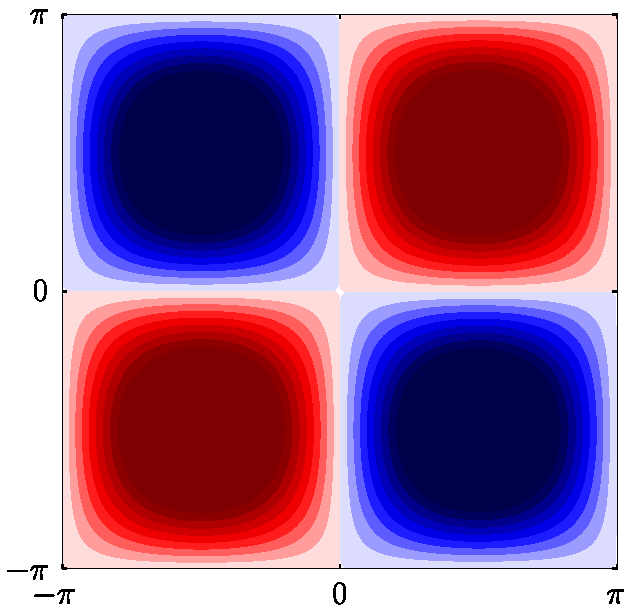
\includegraphics[width=0.42\linewidth]{chapter4/perfect/t-g/3d_vortZ_z=pi4_t=0}
\caption{Taylor--Green vortex initial $\omega_z$ vorticity field at $z=\pi/4$.}
\label{fig:t-g_0}
\end{figure}

\fref{fig:t-g_flow_field} displays how the spanwise-averaged Taylor--Green vortex evolution, governed by the SANS equations, is completely different from the purely 2-D or 3-D turbulence dynamics.
The inclusion of the spanwise stresses (which can be computed in a 3-D simulation) into the 2-D Navier--Stokes solver allows to directly simulate spanwise-averaged dynamics, as demonstrated in \sref{sec:perfect_closure}.
Mathematically, the kinetic energy $\pars{E=1/2\int \vect{u}^2\,\mathrm{d}\Omega}$ and enstrophy $\pars{Z=1/2\int \boldsymbol{\omega}^2\,\mathrm{d}\Omega}$ of 2-D incompressible flows are invariant in the absence of viscosity \citep{Kraichnan1967}, i.e. $\mathrm{D}E/\mathrm{D}t=\mathrm{D}Z/\mathrm{D}t=0$.
This is different in a 3-D system, where the vortex-stretching term $\pars{\boldsymbol\omega\cdot\nabla\vect{u}}$ transfers energy from large scales to small scales of motion inducing local changes in the vorticity field.
In this scenario, enstrophy is no longer conserved and kinetic energy together with helicity $\pars{H=1/2\int \vect{u}\cdot\boldsymbol{\omega}\,\mathrm{d}\Omega}$ are the non-zero quadratic invariants.
Similarly to the vortex-stretching mechanism in 3-D flows, the inclusion of spanwise stresses into the 2-D equations locally adds or removes rotational energy into the system; hence enstrophy and kinetic energy are no longer invariant in the absence of viscosity.

\begin{figure*}
\centering
\setlength{\columnsep}{-0.35cm}
\begin{multicols}{3}
    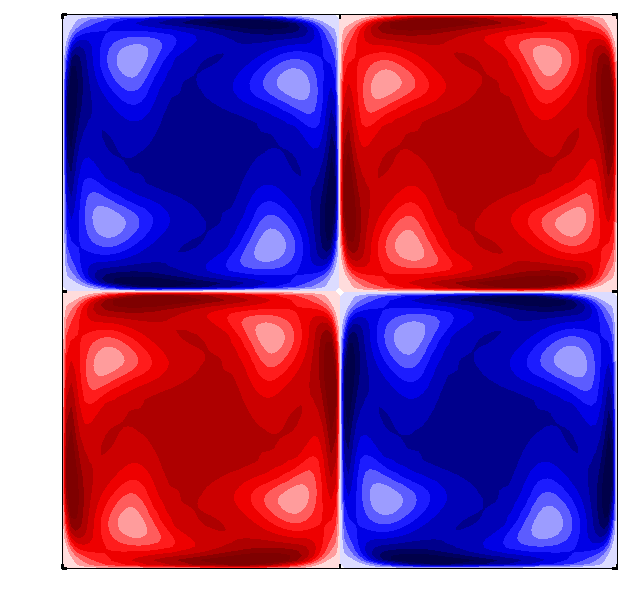
\includegraphics[width=0.9\linewidth]{chapter4/perfect/t-g/3d_vortZ_z=pi_t=81}\par
    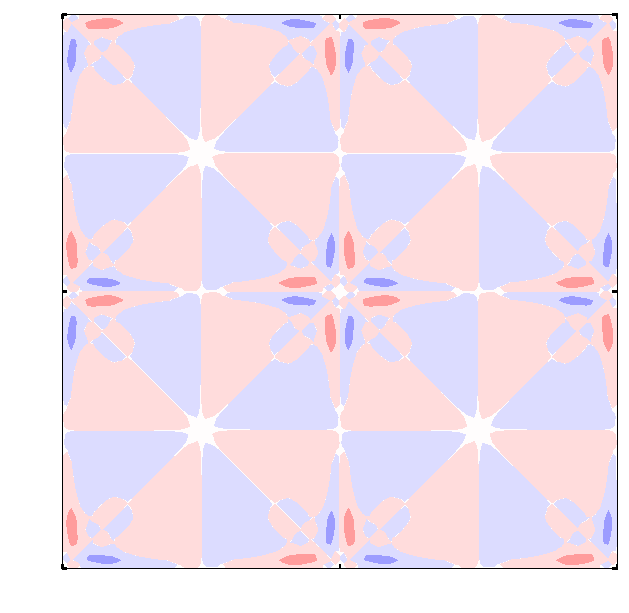
\includegraphics[width=0.9\linewidth]{chapter4/perfect/t-g/3davg_vortZ_t=81}\par
    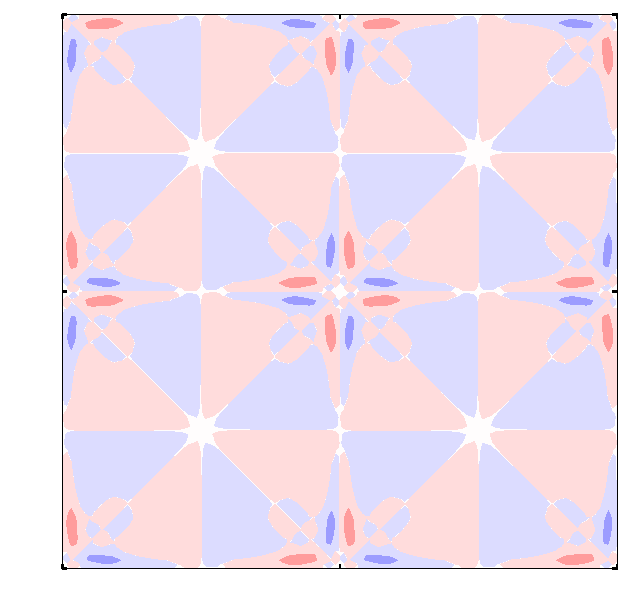
\includegraphics[width=0.9\linewidth]{chapter4/perfect/t-g/2d_vortZ_t=81}\par
\end{multicols}
\vspace{-0.7cm}
\begin{multicols}{3}
    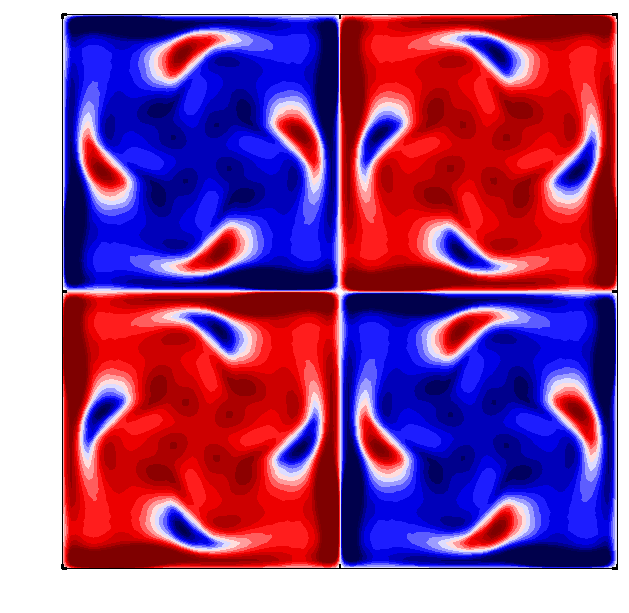
\includegraphics[width=0.9\linewidth]{chapter4/perfect/t-g/3d_vortZ_z=pi_t=122}\par
    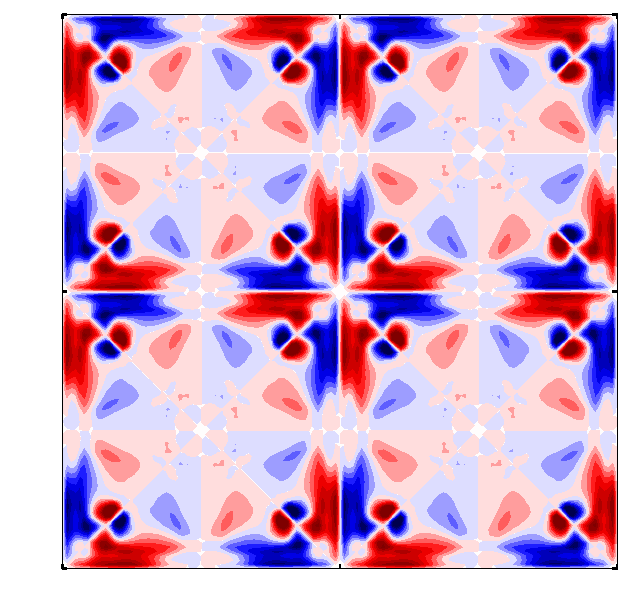
\includegraphics[width=0.9\linewidth]{chapter4/perfect/t-g/3davg_vortZ_t=122}\par
    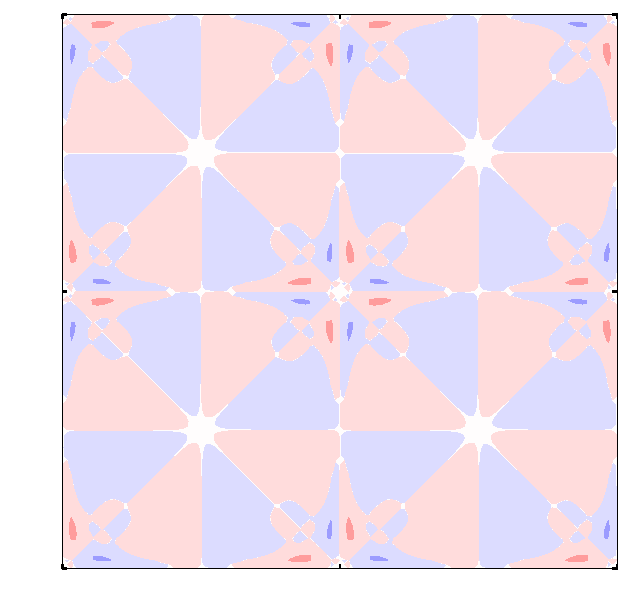
\includegraphics[width=0.9\linewidth]{chapter4/perfect/t-g/2d_vortZ_t=122}\par
\end{multicols}
\vspace{-0.7cm}
\begin{multicols}{3}
    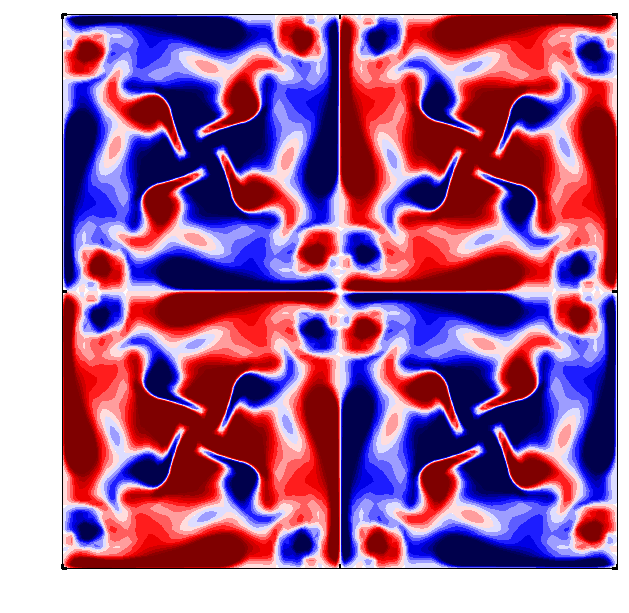
\includegraphics[width=0.9\linewidth]{chapter4/perfect/t-g/3d_vortZ_z=pi_t=163}\par
    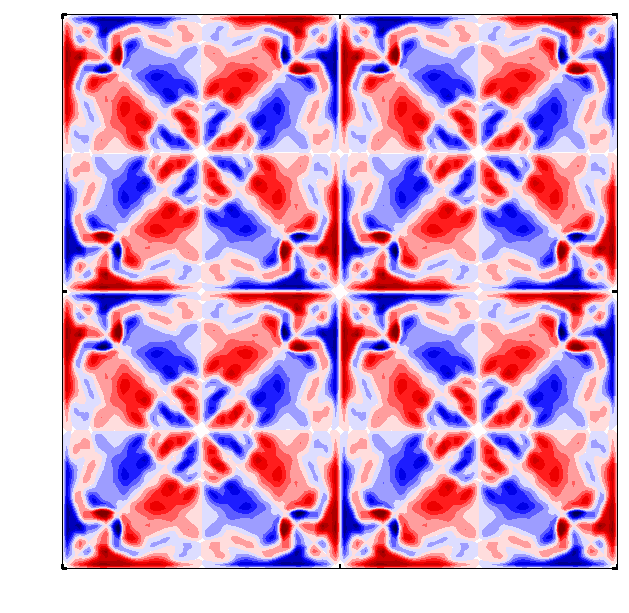
\includegraphics[width=0.9\linewidth]{chapter4/perfect/t-g/3davg_vortZ_t=163}\par
    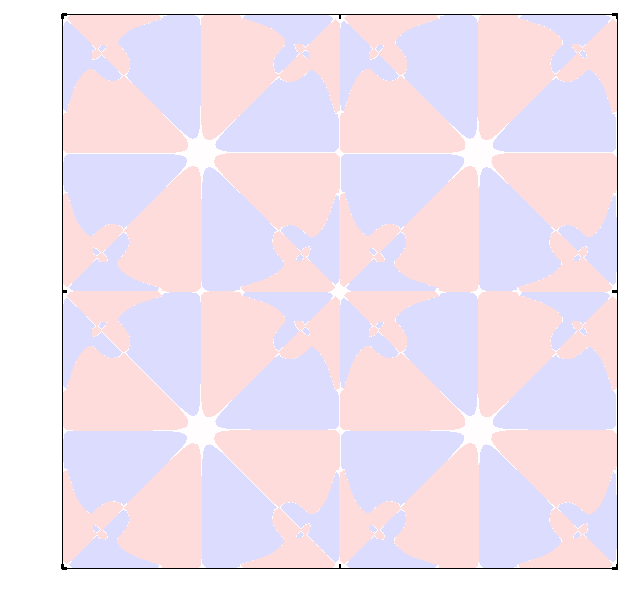
\includegraphics[width=0.9\linewidth]{chapter4/perfect/t-g/2d_vortZ_t=163}\par
\end{multicols}
\vspace{-0.7cm}
\begin{multicols}{3}
    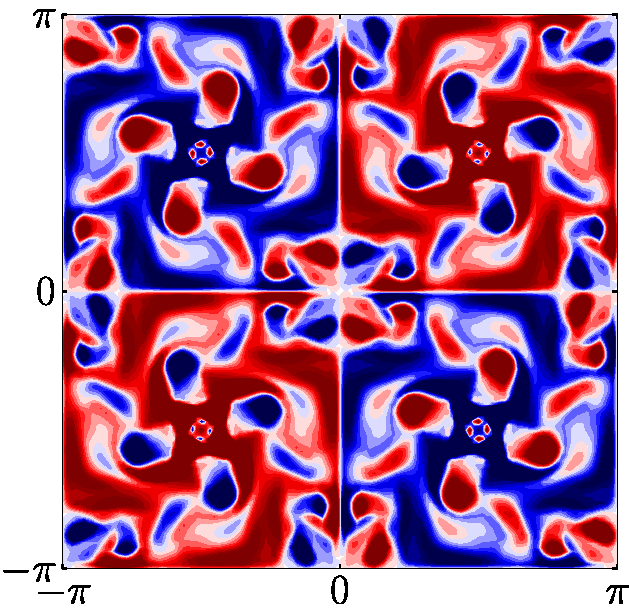
\includegraphics[width=0.9\linewidth]{chapter4/perfect/t-g/3d_vortZ_z=pi_t=203}\par
    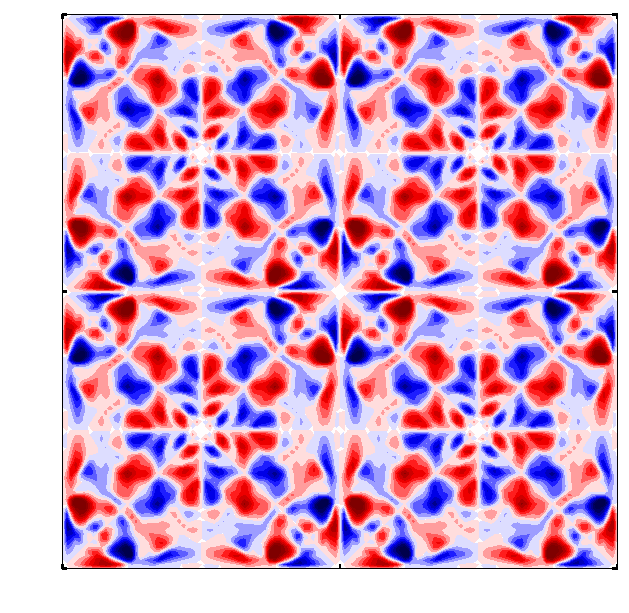
\includegraphics[width=0.9\linewidth]{chapter4/perfect/t-g/3davg_vortZ_t=203}\par
    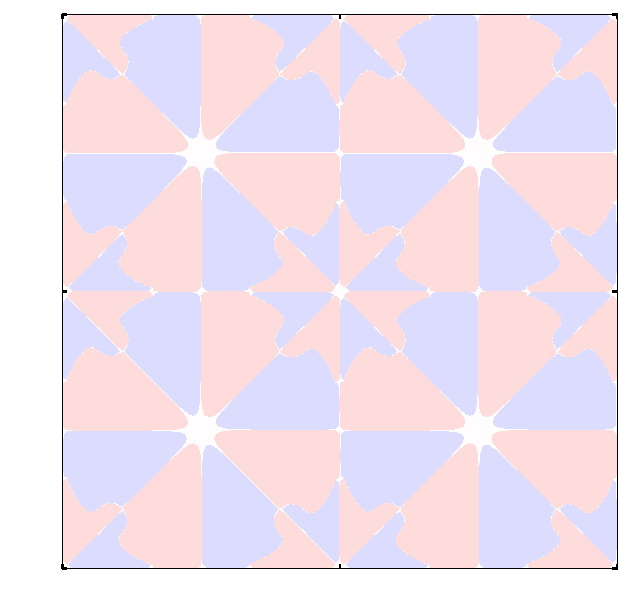
\includegraphics[width=0.9\linewidth]{chapter4/perfect/t-g/2d_vortZ_t=203}\par
\end{multicols}

\caption{Spanwise vorticity evolution of the Taylor--Green vortex at $Re=1600$ in a $2\pi$ periodic box.
From top to bottom: $t^*=4,6,8,10$.
Left: 3-D slice at $z=\pi/4$.
Middle: 3-D spanwise-averaged.
Right: 2-D started from the 3-D spanwise-averaged snapshot at $t^*=4$, where transition to turbulence is expected in the 3-D system.}
\label{fig:t-g_flow_field}
\end{figure*}

\subsection{Perfect closure} \label{sec:perfect_closure}

The SANS equations are numerically verified by including the \textit{perfect closure} of the spanwise stresses in a 2-D simulation.
The perfect closure $(\mathcal{S}^R)$ is defined as the difference between the 2-D Navier--Stokes spatial operator $\tilde{\mathcal{S}}$ and the spanwise-averaged 3-D Navier--Stokes spatial operator $\avg{\mathcal{S}}$.
The inclusion of the perfect closure into the 2-D system allows to calculate the unsteady spanwise-averaged solution of the flow at every time step.
It can be written as
\begin{equation}
\mathcal{S}^R\pars{\vect{u}\p}\equiv \tilde{\mathcal{S}}-\avg{\mathcal{S}},
\label{eq:sans_perfect}
\end{equation}
where
\begin{align}
\mathcal{S}\pars{\vect{u},p}= \vect{u}\cdot\nabla \vect{u} + \nabla p - \nu \nabla^2 \vect{u}, \qquad &\vect{u}=\pars{u,v,w},\,\,\, \vect{x}=\pars{x,y,z},\\
 \tilde{\mathcal{S}}\pars{\vect{U},P}= \vect{U}\cdot\nabla \vect{U} + \nabla P - \nu \nabla^2 \vect{U}, \qquad &\vect{U} = \pars{U,V},\,\,\, \vect{x}=\pars{x,y}.
\end{align}

With the previous definitions, the $\nabla\cdot\boldsymbol\tau_{ij}^R$ closure term in \eref{eq:sans_simple} is redefined as the residual between the operators
\begin{gather}
\partial_t\vect{U}+\tilde{\mathcal{S}}=\tilde{\mathcal{S}}-\avg{\mathcal{S}}\equiv\mathcal{S}^R\pars{\vect{u}\p},\label{eq:perfect_SANS}\\
\partial_t\vect{U}+\tilde{\mathcal{S}}=\mathcal{S}^R.
\end{gather}

Note that, differently from  $\nabla\cdot\boldsymbol\tau_{ij}^R$, the $\mathcal{S}^R$ residual term includes the spatial discretisation error of the resolved spanwise-averaged quantities since $\tilde{\mathcal{S}}$ cancels out in \eref{eq:perfect_SANS} (see \cite{Beck2019} for an analogous explanation for LES closure terms).
Hence, the perfect spanwise-averaged solution can be recovered from the original definition of the SANS equations, i.e. $\avg{\partial_t\vect{u}+\mathcal{S}}=0$.

Beyond the spatial discretisation error inherent in $\nabla\cdot\boldsymbol\tau_{ij}^R$, the quadrature error itself could also affect the perfect recovery of the spanwise-averaged solution.
In this sense, we show in \aref{sec:sans_quadrature_errors1} that the quadrature error for the full SANS equations (\eref{eq:sans_full}) cancels out for the initial state of the Taylor--Green vortex case.
On the other hand, \aref{sec:sans_quadrature_errors2} shows that the quadrature error balance is broken when assuming spanwise periodicity simplifications (\eref{eq:sans_simple}).
Still, the midpoint and trapezoidal quadratures, normally converging with $\mathcal{O}(h^2)$, can achieve exponential convergence rates for periodic functions \citep{Weideman2002,Trefethen2014}.
Hence, the quadrature error should not have a practical impact given it decays faster than the discretisation error of the governing equations.

\subsubsection*{Taylor--Green vortex}

The Taylor--Green vortex flow is used to validate and verify the perfect closure of the SANS equations by computing the closure terms in a 3-D simulation, where their exact solution is known, and then adding them in the 2-D solver at every time step.
We select a uniform resolution of 128 cells in all directions and set $Re=1600$, noting that the purpose of this exercise is to validate the correct derivation of the SANS equations rather than fully resolving the temporal and spatial scales of the problem.
The global kinetic energy and enstrophy are recorded for the spanwise-averaged 3-D,  SANS, and 2-D systems, as displayed in \fref{fig:perfect_t-g}. 
The SANS and 2-D simulations are started from a spanwise-averaged snapshot of the 3-D system at $t^*=4$, where $t^*=t\kappa U_0$.
The evolution of the perfect closure matches the spanwise-averaged 3-D case to machine accuracy.
It can also be observed that energy and enstrophy are not conserved.
Again, this is due to the inclusion of the perfect closure term $(\mathcal{S}^R)$, which changes the system dynamics from standard 2-D Navier--Stokes to SANS.
On the contrary, the 2-D case  almost conserves energy and enstrophy, and the decrease of the metrics is due to viscous and numerical effects.
 
\begin{figure}[!t]
\centering
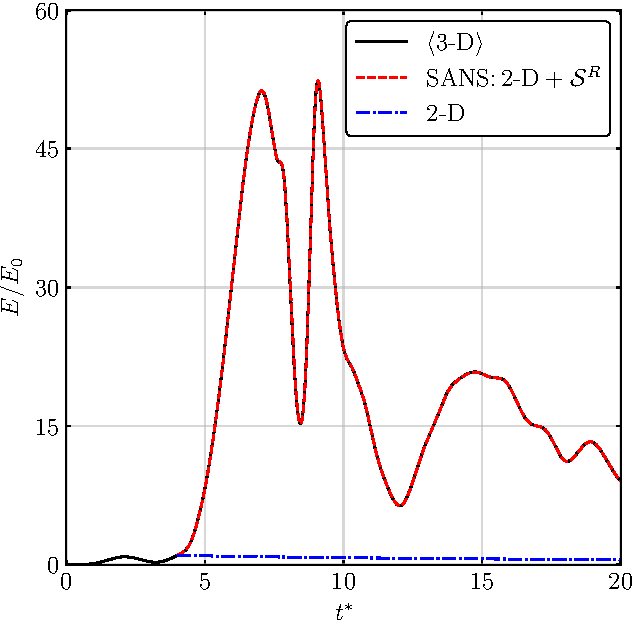
\includegraphics[width=0.48\linewidth]{chapter4/perfect/t-g/E_t0=4}
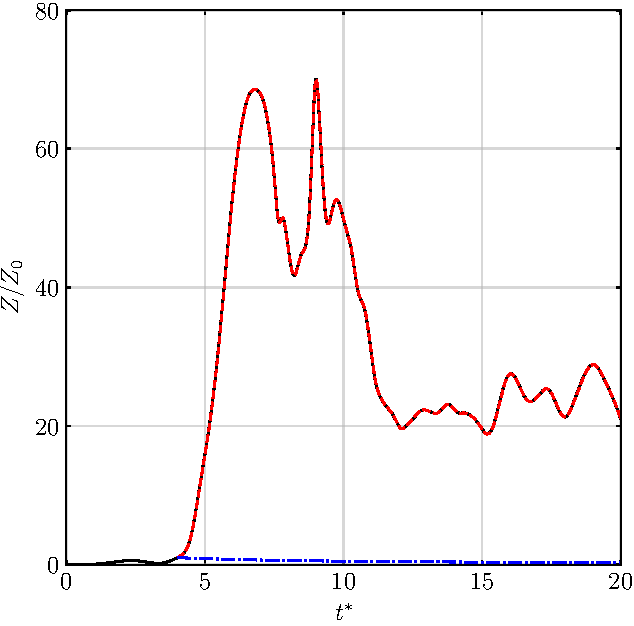
\includegraphics[width=0.48\linewidth]{chapter4/perfect/t-g/Z_t0=4}
\caption{Kinetic energy ($E$, left) and enstrophy ($Z$, right) of the Taylor--Green vortex case.  
$E_0$ and $Z_0$ correspond to the energy and enstrophy at $t^*=4$. 
Energy is computed as $E=1/(2\Omega)\int \vect{U}^2\,\mathrm{d}\Omega$.
Enstrophy is computed as $Z=1/(2\Omega)\int\Omega_z^2\,\mathrm{d}\Omega$, where $\Omega_z=\nabla\times\vect{U}$.}\label{fig:perfect_t-g}
\end{figure}

\begin{figure}[!t]
\centering
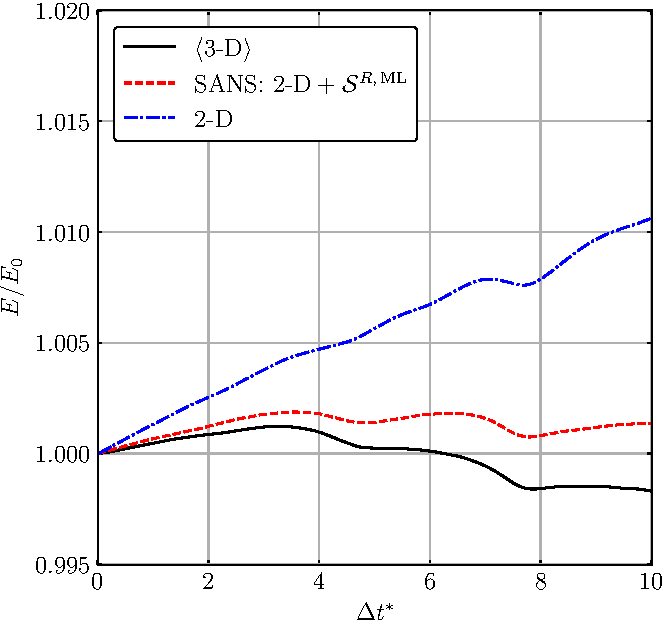
\includegraphics[width=0.50\linewidth]{chapter4/perfect/cc/E}
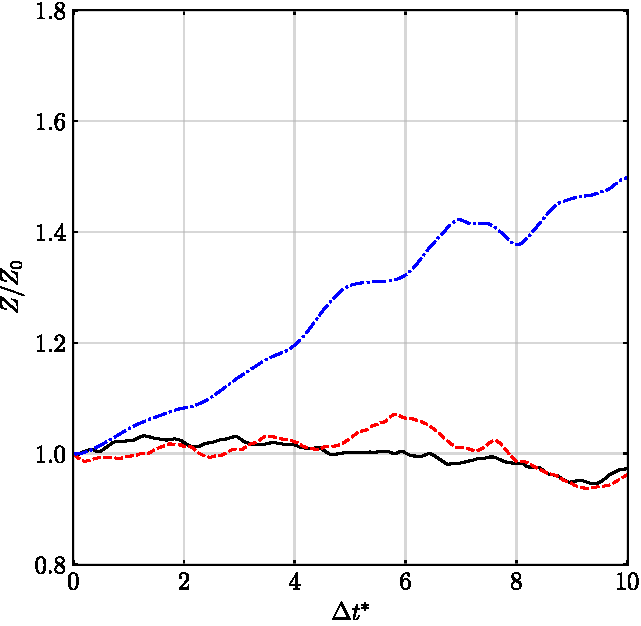
\includegraphics[width=0.48\linewidth]{chapter4/perfect/cc/Z}
\caption{Kinetic energy (left) and enstrophy (right) evolution of flow past a circular cylinder at $Re=10^4$.
$E_0$ and $Z_0$ correspond to the energy and enstrophy at $t_0^*$.
Energy and enstrophy are computed as detailed in \fref{fig:perfect_t-g} caption.}
\label{fig:perfect_cc_EZ}
\end{figure}

\subsubsection*{Flow past a circular cylinder}\label{sec:SANS_circular_cylinder}

Similarly to the Taylor--Green vortex case, the SANS equations are validated with the perfect closure for flow past a circular cylinder at $Re=10^4$.
We employ the same case set-up as \sref{sec:circular_cylinder_details} using a fixed cylinder of $L_z=1$ (span non-dimensionalised with the cylinder diameter).

Starting from a spanwise-averaged 3-D snapshot, the inclusion of the perfect closure in the 2-D solver at every time step allows to recover the unsteady spanwise-averaged flow.
Quantitatively, the difference between the SANS and the 2-D dynamics is emphasised in the kinetic energy and enstrophy evolution (\fref{fig:perfect_cc_EZ}), and the forces induced to the cylinder (\fref{fig:perfect_cc_forces}).
In the 2-D system, both kinetic energy and enstrophy rapidly increase as a result of its natural 2-D system attractor.
On the other hand, the spanwise-averaged dynamics dictate the evolution of the flow when the perfect closure is inserted into the 2-D solution.

Qualitatively, it can be observed in \fref{fig:perfect_cc_vort} that a rapid two-dimensionalisation of the wake develops when the perfect closure is not included in the 2-D solver.
In this scenario, vortical structures are highly coherent after just two convective time units (i.e. $\Delta t^*=t^*-t_0^*=2$, where $t^*=tU/D$).
This is reflected in the over-prediction of the forces induced to the cylinder as a result of the two-dimensionalisation mechanism yielding energised vortices in the near wake region.

The over-prediction of the hydrodynamic forces is the main short-coming of standard 2-D strip-theory methods, which arbitrarily include additional dissipation mechanisms such as 2-D turbulence models to tackle this issue.
Here we show that correctly modelling the SSR terms can bypass this problem by explicitly including 3-D effects into the governing equations while keeping the low computational cost of 2-D strip-theory methods.

\begin{figure}[!t]
\centering
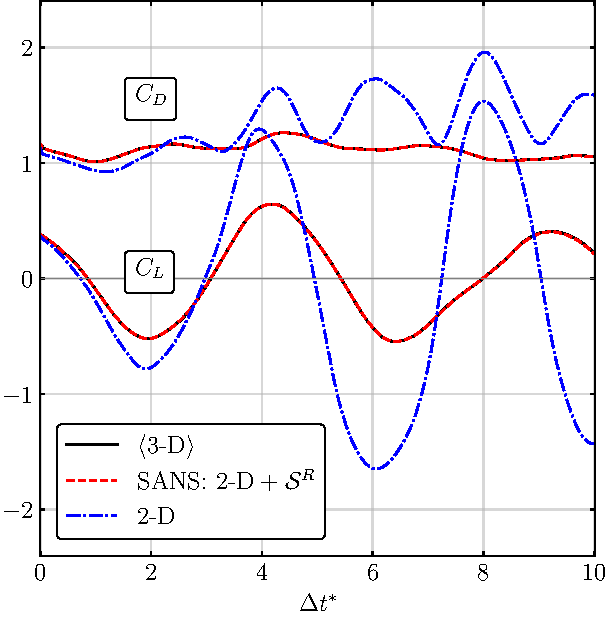
\includegraphics[width=0.48\linewidth]{chapter4/perfect/cc/forces}
\caption{Lift (bottom) and drag (top) force coefficients of flow past a circular cylinder at $Re=10^4$.
The force coefficients in the 3-D system have been calculated as $C_{L,D}=2F_{y,x}/(\rho U_\infty^2 D L_z)$, where $F_y$ and $F_x$ are respectively the vertical and horizontal pressure force, $\rho$ is the constant density, $U_\infty$ is the free-stream velocity, and $D$ is the cylinder diameter.
The force coefficients in the 2-D system are calculated analogously without factoring by $1/L_z$.}
\label{fig:perfect_cc_forces}
\end{figure}

\begin{figure}[!t]
    \centering
    \begin{subfigure}[t]{0.7\linewidth}        
        \centering
        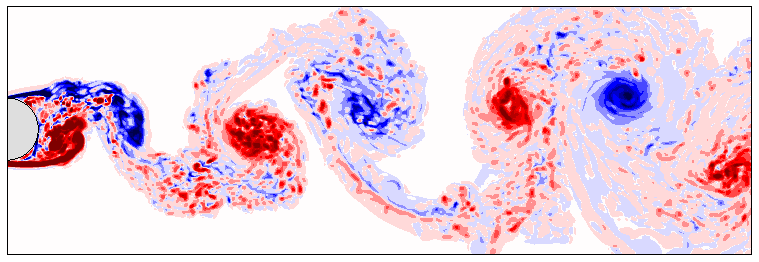
\includegraphics[width=\linewidth]{chapter4/perfect/cc/3-D_t=3700_lowres}
        \caption{$\avg{3\text{-}\mathrm{D}}$, $t^*_0$.}\vspace{0.4cm}
    \end{subfigure}
    \begin{subfigure}[t]{0.7\linewidth}
        \centering
        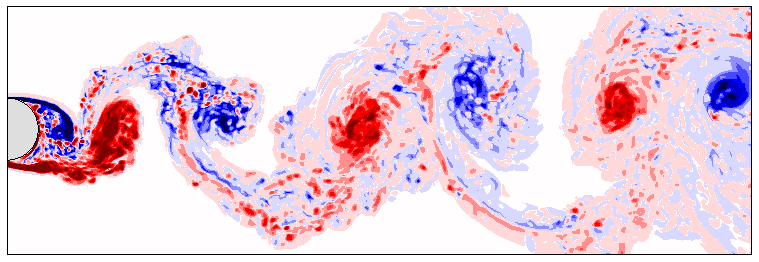
\includegraphics[width=\linewidth]{chapter4/perfect/cc/3-D_t=3702_lowres}
        \caption{SANS: $2\text{-}\mathrm{D}+\mathcal{S}^{R}$, $\Delta t^*=2$.}\vspace{0.4cm}
    \end{subfigure}
    \begin{subfigure}[t]{0.7\linewidth}
        \centering
        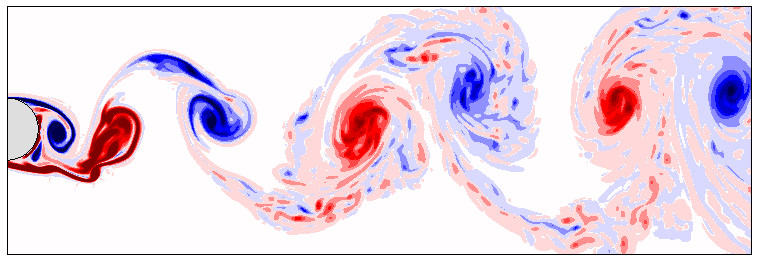
\includegraphics[width=\linewidth]{chapter4/perfect/cc/2-D_t=3702_lowres}
        \caption{$2\text{-}\mathrm{D}$, $\Delta t^*=2$.}
    \end{subfigure}
    \captionsetup[subfigure]{width=\linewidth}
    \caption{Top: Vorticity of the spanwise-averaged 3-D flow used as initial condition for the SANS and the 2-D simulations.
Middle: Vorticity obtained in the SANS system after 2 convective time units.
Bottom: Vorticity obtained in the 2-D system after 2 convective time units.}
\label{fig:perfect_cc_vort}
\end{figure}

\subsection{Eddy-viscosity model} \label{sec:evm}

The most common model for the closure terms arising from time-averaged (RANS) or spatially-filtered (LES) Navier--Stokes equations is based on the eddy-viscosity (Boussinesq) hypothesis.
Under this hypothesis, it is assumed that the unresolved scales of motion can be linked to an effective (positive scalar) viscosity additional to the molecular viscosity of the fluid.
This implies that the closure terms can only have a dissipative effect in the governing equations.
Analogous to the definition of the stress tensor for Newtonian fluids, the eddy-viscosity hypothesis is defined as
\begin{equation}
\boldsymbol\tau^r_{ij}\equiv\avg{\vect{u}\p\otimes\vect{u}\p}-\frac{2}{3}k\delta_{ij}=-2\nu_t \avg{S_{ij}},
\label{eq:Boussinesq}
\end{equation}
where $\boldsymbol\tau^r_{ij}$ is the anisotropic SSR tensor, $\avg{S_{ij}}=(\nabla\otimes\avg{\vect{u}}+\avg{\vect{u}}\otimes\nabla)/2$ is the mean rate-of-strain tensor, $\nu_t$ is the eddy viscosity, $k=\mathrm{tr}\avg{\vect{u\p}\otimes\vect{u\p}}/2$ is the turbulence kinetic energy, and $\delta_{ij}$ is the Kronecker delta tensor.
The following relations arise for 2-D incompressible flow
\begin{gather}
\avg{u\p u\p}-2k/3=-2\nu_t\partial_x U,\label{eq:evm1}\\
\avg{v\p v\p}-2k/3=-2\nu_t\partial_yV,\\
\avg{u\p v\p}=-\nu_t\pars{\partial_yU+\partial_xV}.\label{eq:evm3}
\end{gather}

The eddy-viscosity field in \eref{eq:Boussinesq} has been a subject of research for decades and many different eddy-viscosity models (EVMs) have been developed for RANS and LES flow descriptions.
One of the most successful is the LES Smagorinsky model \citep{Smagorinsky1963}
\begin{equation}
\nu_t=\pars{C_s \Delta}^2\sqrt{2\avg{S_{ij}}\avg{S_{ij}}},
\end{equation}
where $\Delta$ is the averaging filter width, and $C_s$ is the Smagorinsky constant which tunes the amount of SGS kinetic energy to be removed.

\subsubsection*{A-priori results} \label{sec:EVM_a-priori}

To test the applicability of EVMs for SANS flow, we apply the Smagorinsky model to the circular cylinder flow field, manually selecting the value of $C_s$ to provide the best magnitude fit with the anisotropic part of the residual tensor.
As this a-priori assessment assumes knowledge of the best $C_s$ and does not require any modelling of the isotropic part of the stress tensor (i.e. the SSR kinetic energy, $k$), it represents the best possible results for the EVM\footnotemark.
In the context of this work and as often found in the literature, \textit{a-priori} analysis refers to the analysis of the model performed before deploying it in a live simulation.
Such analysis uses reference data previously generated with the full system of equations, i.e. the 3-D Navier--Stokes equations.
On the other hand, \textit{a-posteriori} analysis refers to the deployment of the trained model in a live 2-D simulation, where metrics such as the unsteady hydrodynamic forces can be used as a performance indicator of the model.

\footnotetext{In an a-posteriori framework, turbulence modelling requires the full residual stress tensor to solve the averaged governing equations. Hence, EVMs usually incorporate the isotropic part $\pars{2k/3}$ in the total pressure defining a new pressure field, $p^*=p+2k/3$, on which a divergence-free velocity field is projected.
Alternatively, a transport equation for the TKE can also be considered.}

The a-priori correlation of the EVM as defined by the Boussinesq hypothesis (Eqs. \ref{eq:evm1} to \ref{eq:evm3}) is displayed in \fref{fig:evm_density_plots} in terms of density plots, where the eddy-viscosity field is not accounted yet.
The observed density distributions hint that a closure based on the eddy-viscosity hypothesis will most likely fail to correctly capture the SSR anisotropic tensor components.
This arises from the fact that no eddy-viscosity field (scalar) will be able map the resolved quantities to the different components of the closure tensor, as the density plot is significantly different between normal and shear components.

\begin{figure}[!t]
\centering
    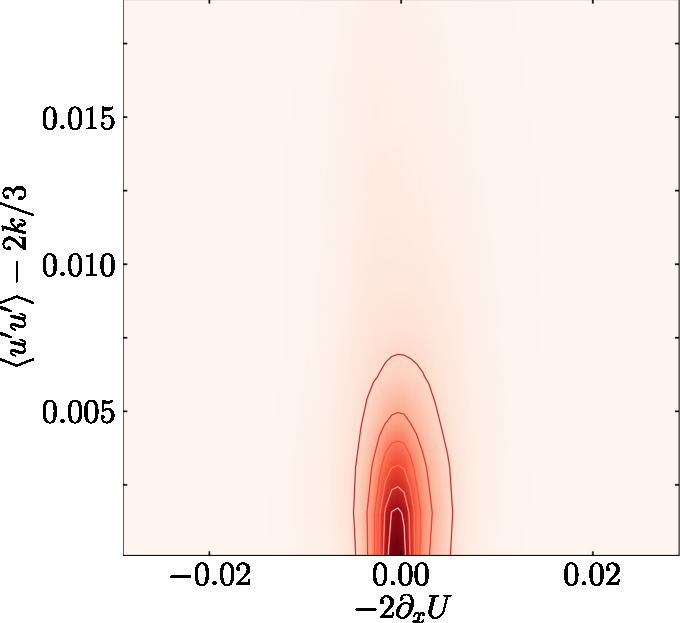
\includegraphics[width=0.45\linewidth]{chapter4/evm/density_plots/uu-dUdx_dens_detail_lowres.pdf}\hspace{1em}
    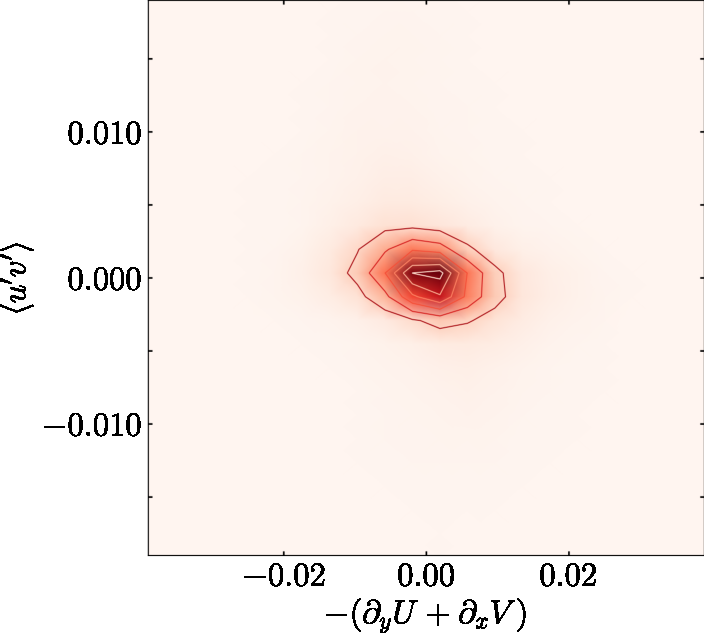
\includegraphics[width=0.45\linewidth]{chapter4/evm/density_plots/uv-dUdy+dVdx_dens_detail_lowres.pdf}
\caption{Density plots of the Boussinesq relationship between resolved and fluctuating quantities computed within the $x \in [0, 12], y \in [-2, 2]$ domain of the cylinder wake.}
\label{fig:evm_density_plots}
\end{figure}

The a-priori results of the EVM with the Smagorinsky closure are shown in \fref{fig:EVM_a-priori}.
Almost no qualitative similarity with the target components of the SSR anisotropic tensor can be observed, thus evidencing the poor performance of the EVM on capturing the spanwise fluctuations.
This poor performance is quantified in \tref{tab:a-priori_EVM} using the Pearson correlation coefficient
\begin{equation}
\mathcal{CC}\pars{\boldsymbol\tau^r_{ij},\boldsymbol\tau^{r,\,\mathrm{EVM}}_{ij}}=\frac{\mathrm{cov}\pars{\boldsymbol\tau^r_{ij},\boldsymbol\tau^{r,\,\mathrm{EVM}}_{ij}}}{\sqrt{\mathrm{cov}\Big(\boldsymbol\tau^r_{ij},\boldsymbol\tau^r_{ij}\Big)\mathrm{cov}\pars{\boldsymbol\tau^{r,\,\mathrm{EVM}}_{ij},\boldsymbol\tau^{r,\,\mathrm{EVM}}_{ij}}}},
\end{equation}
where the superscript $(\cdot)^{\mathrm{EVM}}$ denotes the EVM prediction.
The low correlation values provide clear evidence that the EVM is not suited for the prediction of the spanwise stresses.

These poor results are ultimately expected since EVMs only account for the dissipative effects of turbulent fluctuations.
In the spanwise-averaged system, the spanwise stresses can have both a dissipative and energising physical effect, and this is a fundamental difference which no EVM can reproduce.

\begin{table}[t]
\centering
\caption{Correlation coefficients between components of the target anisotropic SSR tensor and predictions provided by the EVM.}
\begin{tabular}{lrrr}
\toprule
$\mathcal{CC}$ & $\boldsymbol\tau^r_{11}$ & $\boldsymbol\tau^r_{12}$ & $\boldsymbol\tau^r_{22}$ \\
\midrule
EVM &  0.06& 0.06 & 0.14\\
\bottomrule
\label{tab:a-priori_EVM}
\end{tabular}

{\footnotesize The correlation coefficients are calculated for 500 snapshots and the average values are provided. \par}
\end{table}

\begin{figure}[!ht]
\centering
\begin{subfigure}[t]{0.6\linewidth}
    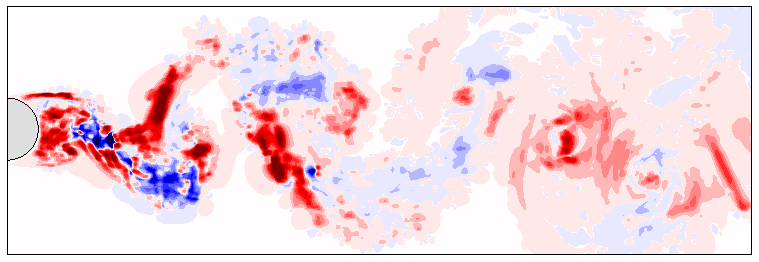
\includegraphics[width=\linewidth]{chapter4/evm/a-priori/tau_r_11_lowres}
    \caption{$\boldsymbol\tau^r_{11}$} 
\end{subfigure}
\begin{subfigure}[t]{0.6\linewidth}
    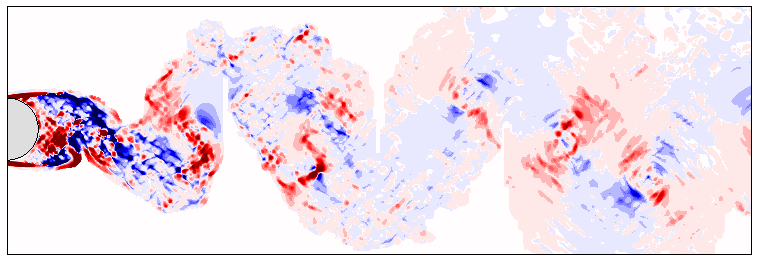
\includegraphics[width=\linewidth]{chapter4/evm/a-priori/tau_r_11_EVM_lowres}
    \caption{$\boldsymbol\tau^{r,\,\mathrm{EVM}}_{11}$}
\end{subfigure}
\begin{subfigure}[t]{0.6\linewidth}
    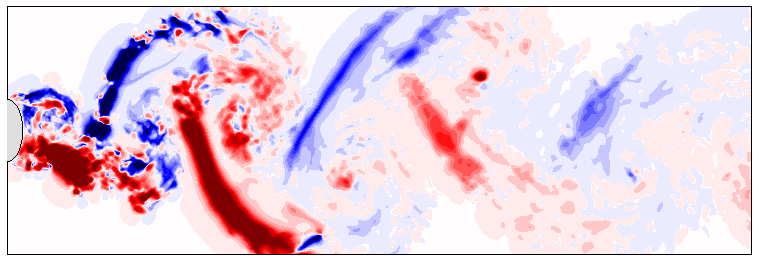
\includegraphics[width=\linewidth]{chapter4/evm/a-priori/tau_r_12_lowres}
    \caption{$\boldsymbol\tau^r_{12}$}
\end{subfigure}
\begin{subfigure}[t]{0.6\linewidth}
    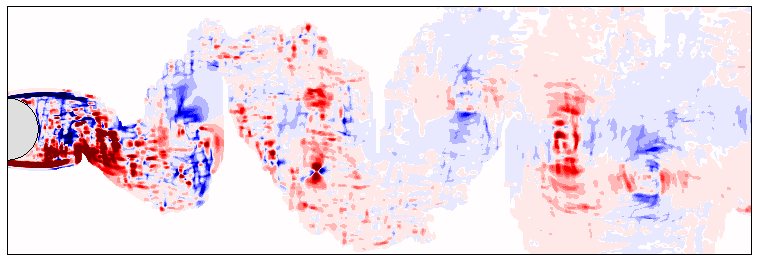
\includegraphics[width=\linewidth]{chapter4/evm/a-priori/tau_r_12_EVM_lowres}
    \caption{$\boldsymbol\tau^{r,\,\mathrm{EVM}}_{12}$}
\end{subfigure}
\begin{subfigure}[t]{0.6\linewidth}
    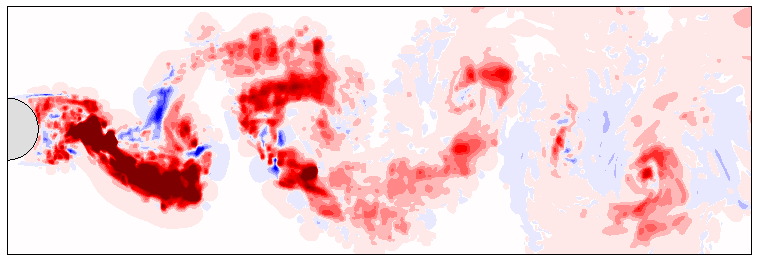
\includegraphics[width=\linewidth]{chapter4/evm/a-priori/tau_r_22_lowres}
    \caption{$\boldsymbol\tau^r_{22}$}
\end{subfigure}
\begin{subfigure}[t]{0.6\linewidth}
    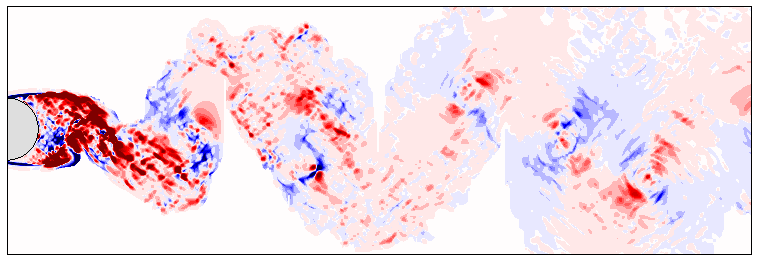
\includegraphics[width=\linewidth]{chapter4/evm/a-priori/tau_r_22_EVM_lowres}
    \caption{$\boldsymbol\tau^{r,\,\mathrm{EVM}}_{22}$}
\end{subfigure}
\caption{EVM predictions of the anisotropic SSR tensor components $(\boldsymbol\tau^{r,\,\mathrm{EVM}}_{ij})$ compared to reference data $(\boldsymbol\tau^{r}_{ij})$.}
\label{fig:EVM_a-priori}
\end{figure}

\clearpage
\section{Conclusion}

A flow decomposition based on the local spanwise average has been proposed  aiming to reduce the system dimensionality of flows presenting an homogeneous direction.
The SANS equations yield the spanwise-averaged solution of a 3-D flow in a 2-D system.
In practical terms, the SANS equations are equivalent to the incompressible 2-D Navier--Stokes equations with additional forcing terms representing the spanwise fluctuating part of the flow.

First, we examine the SANS equations in an analytical test case consisting in the superposition of a vortex tube and a straining field.
It is demonstrated that the SANS equations still include the vortex-stretching mechanism.
On the other hand, the SANS equations are greatly simplified when the flow is assumed to be spanwise periodic.
The vortex-stretching term plus other terms arising from averaging over a finite non-periodic interval vanish as a result of this constraint.

In spanwise-periodic conditions, the SANS equations only contain the divergence of the SSR tensor as a closure term.
In this sense, the perfect closure is presented as the difference between the 2-D Navier--Stokes spatial operator and the spanwise-averaged 3-D Navier--Stokes spatial operator.
The SANS equations are validated by incorporating the perfect closure term computed in a 3-D system into a 2-D simulation.
This allows to recover the unsteady spanwise-averaged solution of a Taylor--Green vortex and flow past a circular cylinder at $Re=10^4$.
The inclusion of the perfect closure radically changes the flow dynamics, where energy and enstrophy are no longer conserved in the inviscid limit.

Finally, an EVM has been investigated to provide closure to the SANS equations for the cylinder flow test case.
The a-priori analysis has shown that the Boussinesq hypothesis completely fails to capture the nature of the closure terms.
This underlines the need for a different SANS model bearing in mind that, differently from RANS or LES, general information on the physical laws governing the closure terms is still limited.
The possibility of directly computing the closure terms in 3-D systems can be exploited with the use of data-driven models such as machine-learning algorithms, as reviewed in the following chapter.
% ---------------------------------------------------------------- 
\end{document}

